\documentclass[11pt]{beamer}
\usepackage[utf8]{inputenc}
\usepackage{hyperref}
\usepackage{amsmath,amsthm, amssymb, latexsym,amsfonts,pgf}
\usecolortheme{seahorse}
\usepackage{lmodern}
\usepackage{tabularx}
\usepackage{array}
\usepackage{xcolor}
\usepackage{tikz}
\usepackage{graphicx} % to include images
\usepackage{booktabs} % Allows the use of \toprule, \midrule and \bottomrule in tables
\setbeamercovered{transparent}
\usetheme{CambridgeUS}

%\usecolortheme{albatross}
%\usecolortheme{beaver}
%\usecolortheme{beetle}
%\usecolortheme{crane}
%\usecolortheme{dolphin}
%\usecolortheme{dove}
%\usecolortheme{fly}
%\usecolortheme{lily}
%\usecolortheme{orchid}
%\usecolortheme{rose}
%\usecolortheme{seagull}
%\usecolortheme{seahorse}
%\usecolortheme{whale}
%\usecolortheme{wolverine}
\usepackage{newtxtext,newtxmath}
\setbeamertemplate{headline}
{
  \leavevmode%
  \hbox{%
  \begin{beamercolorbox}[wd=.5\paperwidth,ht=2.25ex,dp=1ex,right]{section in head/foot}%
   \usebeamerfont{section in head/foot}\thesection.\ \insertsectionhead\hspace*{2ex}
  \end{beamercolorbox}%
  \begin{beamercolorbox}[wd=0.5\paperwidth,ht=2.25ex,dp=1ex,left]{subsection in head/foot}%
    \usebeamerfont{subsection in head/foot}\hspace*{2ex}\insertsubsectionhead
  \end{beamercolorbox}}%
  \vskip0pt%
}
\title[A Study on Self-similar Tilings]{ Topological properties of tiles related to number systems  }
\author[Angel Meera]{\textbf {Angel Meera}\\ {(RMM21201)} \\
\vspace{0.2cm}Under the supervision of\\\vspace{0.2cm} Dr.  }
\institute[IIITL]{\large{\small  Indian Institute of Information Technology,  Lucknow}\vspace{0.5cm}}
\logo{
\includegraphics[width=1cm]{iiitl.png}}
\date[Today]{\today} %{17 January 2023}
\AtBeginSection[]
 

\begin{document}


\maketitle

\begin{frame}{Overview}
\tableofcontents
\end{frame}

\section{Introduction}
\begin{frame}{Introduction}
    \begin{itemize}
        \item  Mandelbrot started his work with those now famous words:\\
    \begin{center}
    \textit{"Clouds are not spheres, mountains are not circles,  and bark is not smooth, nor does lightning travel in a straight line".}
    \end{center}
        \pause 
        \item Geometric
        \pause 
        \item
        \item 
    \end{itemize}
    
\begin{figure}
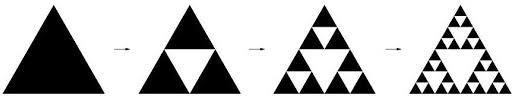
\includegraphics[height=2cm]{Sier.jpg}
\caption{}
\end{figure}
\end{frame}



\begin{frame}{Motivation}
\section{Motivation}
\begin{block}
    
C. Bandt formulated the theory based on crystallographic structures. The motivation to this paper is to reproduce the same theory in tiles using some mathematical theories. 
 \end{block}   
\end{frame}


\subsection{Related Work}
    \begin{frame}{ Related Work}
\begin{itemize}
\item There is a discussion on
\item 
\item 
\item 
\end{itemize}
\end{frame}


\section{Literature Survey}
\begin{frame}{Summary}
       \begin{center}

\scriptsize \begin{tabular}{|p{0.4cm}|p{1.0cm}|p{1.7cm}|p{1.2cm}|p{1.7cm}|p{2cm}|}
 \hline
 \textbf{S. No.} & \textbf{Authors and Year} & \textbf{Problem Statement} & \textbf{Method} & \textbf{Findings} & \textbf{Limitations}\\ 
 \hline
 \cite{1}  & Bandt et al., 2019 &  &  &  & \\
 \hline
 \cite{2} &  &  &  &  & \\
 \hline
 \cite{3} &  &  &  &  & \\
 \hline
 \cite{4} &  &  &  &  & \\
 \hline
 \cite{5} &  &  &  &  & \\
 \hline

\end{tabular}
\end{center}

\end{frame}

\section{Research Problem}
\begin{frame}{Problems}
    \begin{enumerate}
        \item  
        \item 
        \item 
        \item
    \end{enumerate}
\end{frame}


\section{Future Scope}
\begin{frame}{Future Scope}
\begin{itemize}
    \item 
    \item 
\end{itemize}
 \end{frame}

 \section{Conclusion}
\begin{frame}{Conclusion}
The first objective of extending the topological study of a family of tiles to higher dimensional cases may be proved by the contact matrix approach. Some results were observed from geometric substitution tilings. We have also tried solving using the method of combinatorial substitutions as well.
\end{frame}


\section{References}
\begin{frame}{References}
    \begin{thebibliography}{111}

\bibitem{m}

\bibitem{1}  S. Akiyama, J. M Thuswaldner, \textit{A survey on topological properties of tiles related to number systems}, Geometriae Dedicata volume 109, pages 89–105 (2004)  

\bibitem{2} 

\bibitem{3}

\end{thebibliography}
\end{frame}

\begin{frame}
 \begin{thebibliography}{111}
\bibitem{4} 

\bibitem{5} 

\bibitem{6} 

\end{thebibliography}
\end{frame}

\section{}
 \begin{frame}{}
  \centering \Huge  \textbf{Thank You!}
\end{frame}

\end{document}